\section{Introduction}
% \subsection{X-ray fluorescence data acquisition method}
\subsection{Motivation}
The work presented is built upon contributions made by dr. inż. Bartłomiej Łach in his doctoral thesis entitled ``Rozwój systemu detekcyjnego do obrazowania przestrzennego rozkładu pierwiastków metodą fluorescencji rentgenowskiej'' \cite{Lach2022}  (eng. \emph{Development of a detection system for spatial imaging of element distribution using X-ray fluorescence}).

His dissertation was dedicated to development of system for non-invasive analysis of works of art that uses X-ray radiation to carry out measurements. 
The system presented was designed to provide a map of element distribution in the top layers of the object, offering essential information for analyzing the pigments used in the artwork. 
The results provided by analysis could be source of important knowledge for conservators of monuments and art, informing them about the object's state of preservation, quality of past maintenance processes, the work's authenticity and leading to the expansion of previous state of knowledge.

The most popular technique to perform measurements, namely MA-XRF (Macro X-Ray Fluorescence), operate by scanning selected parts of art point by point. 
This method is characterized by high spatial and energetic resolution. 
However, due to usage of polycapillary lenses it is limited to performing scans on 2D surfaces.
Another drawback this method shows is long measurement time. 

An alternative method involves scanning not just a single point but multiple points within a specified area of the surface, by utilizing FF-XRF (Full-Field X-Ray Fluorescence). 
This exact approach was implemented by researchers at AGH University of Krakow in the DETART (Detector for Art) data acquisition system. 
DETART not only can scan large portion of the surface (over $10^5$ pixels at the same time), but it is also capable of performing scans of 3D objects without losing spatial resolution thanks to (theoretically) near infinite depth of field provided by pinhole camera. 

After data acquisition part, the analysis can be performed. 
Łach proposed three different methods for analyzing data: ``standard'' ROI (Region Of Interest) method and two different machine learning algorithms: PCA (Principal Components Analysis) and NFM (Non-negative Matrix Factorization). 
Each of them had its advantages and disadvantages. 
In the end, there may not be a single method that is universally superior. 
However, employing multiple methods allows us to draw more comprehensive conclusions, leveraging the strengths of each and compensating for their respective limitations.

\subsection{Concept}
Concept of this thesis is heavily inspired by the work presented in \cite{Jones2022}. 
The authors of this article introduced the idea of a CNN (Convolutional Neural Network) model tasked with classifying every sample measured with XRF as one pigment class. 
Researchers trained the model on synthetic data first, achieving through it an accuracy of 55\% after performing tests on real XRF spectra, and 96\% after applying transfer learning using small quantity of real XRF samples.  
This approach is pretty convenient for further usage thanks to full automation of the process. 
It also presents high accuracy after application of transfer learning.
However, there are some downsides to consider:
\begin{itemize}
    \item The model can only classify pigments it has learned about
    \item It does not provide any information about signals coming from elements, which may offer some valuable insights about the studied object
\end{itemize}
A potential solution to these problems may be to shift the focus from classifying pigments to classifying elements. A multi-label classification approach might be used to assess existence of each learned element independently from the tested pigment. This approach is more similar to algorithms used in Łach's thesis.

\subsection{Introduction to XRF}
\subsubsection{Physics fundations}
XRF method utilizes X-ray radiation to provide data for further analysis of objects exposed to radiation. 
It is considered harmless when used in small doses and low intensity.  
Therefore, it can be used to study delicate objects, such as art, monuments, geological and biological samples.
Characteristic X-ray fluorescence radiation is type of secondary radiation generated in matter under the influence of radiation from an external source - X-ray tube in research setting.

The fundamental physics behind the whole process is the phenomenon of photoelectric absorption.
In this process, one of photons transfers all its energy to one of the electrons bound to the inner electron shell of an atom. 
Consequently the electron is ``knocked out'' from its position on the shell, leaving a vacant space (hole) in the shell. 
Absorption can only occur if the energetic criterion is satisfied; that is, the energy that photon gives to the electron must be greater than the binding energy of electron in the specific shell.

After the emission of the electron, the state of the atom is unstable (excited), which results in electron jumping from a higher level to the vacancy left by the emitted electron, creating its own vacancy.
The entire process continues until the atom reaches an equilibrium state.

Electrons placed on outer shells have higher energies than electrons on lower shells. 
According to the law of conservation of energy, something must happen to the excess energy - the emission in the form of characteristic photon occurs. 
The binding energies on each shell are unique features of every element and are related to the energies of characteristic photons.
These energies are also known as spectral lines. 
For example, when an electron jumps from shell L to K, it releases energy equal to the difference between their binding energies, resulting in the K$_\alpha$ spectral line. 
Similarly, when it jumps from shell M to K, it produces the K$_\beta$ spectral line, and so on.
Therefore, with \emph{a priori} knowledge about energies of specific spectral lines, one should be able to identify elements present in measured spectrum - see \prettyref{fig:photons_energy}.

\begin{figure}[h] 
  \centering     
   \begin{overpic}[width=0.8\linewidth]{img/dependence_of_photons_energy.png}
    \put(-3,18){\rotatebox{90}{\textcolor{black}{Photon energy [KeV]}}}
    \put(35,-3){\textcolor{black}{Atomic number Z [-]}}
  \end{overpic}
  \vspace{10pt}
  \caption{The dependence of the energy [KeV] of photons  emitted due to transitions of electrons from the L to K level (K$_\alpha$ spectral line) and M to L level (L$_\alpha$ spectral line) as a function of the atomic number Z [-]. Source: \cite{Lach2022}} 
  \label{fig:photons_energy}
\end{figure}

At the same time competitive process can occur - Auger electron ejection. This process involves the following events\cite{augerElectron}:
\begin{enumerate}
    \item An electron on the inner shell is ejected by a photon, creating a vacancy.
    \item A secondary electron drops down to fill the vacancy.
    \item If sufficient energy is emitted, a tertiary electron is ejected (Auger electron)
\end{enumerate}
For example, vacancy may be created on shell K, leading to transition from shell L to K and then emission of Auger electron from shell L (or M, or any higher).
Emission of these electrons is an undesirable effect in context of XRF, as it is responsible for the presence of background in the measured spectrum.

\subsubsection{Imaging techniques}
XRF is primarily employed for quantitative measurements of elements in studied samples. 
Handheld scanners with high energy resolution are available on the market, suitable for simple measurements of elements present in metal alloys, geodes and other materials. 
However, if one is interested in spatial imaging, device like that will (probably) not suffice. 
The demand for spatial imaging led to the evolution of X-ray scanning microscopy - \prettyref{fig:ma-xrf}

\begin{figure}[h] 
  \centering     
      \begin{subfigure}{0.45\linewidth}
      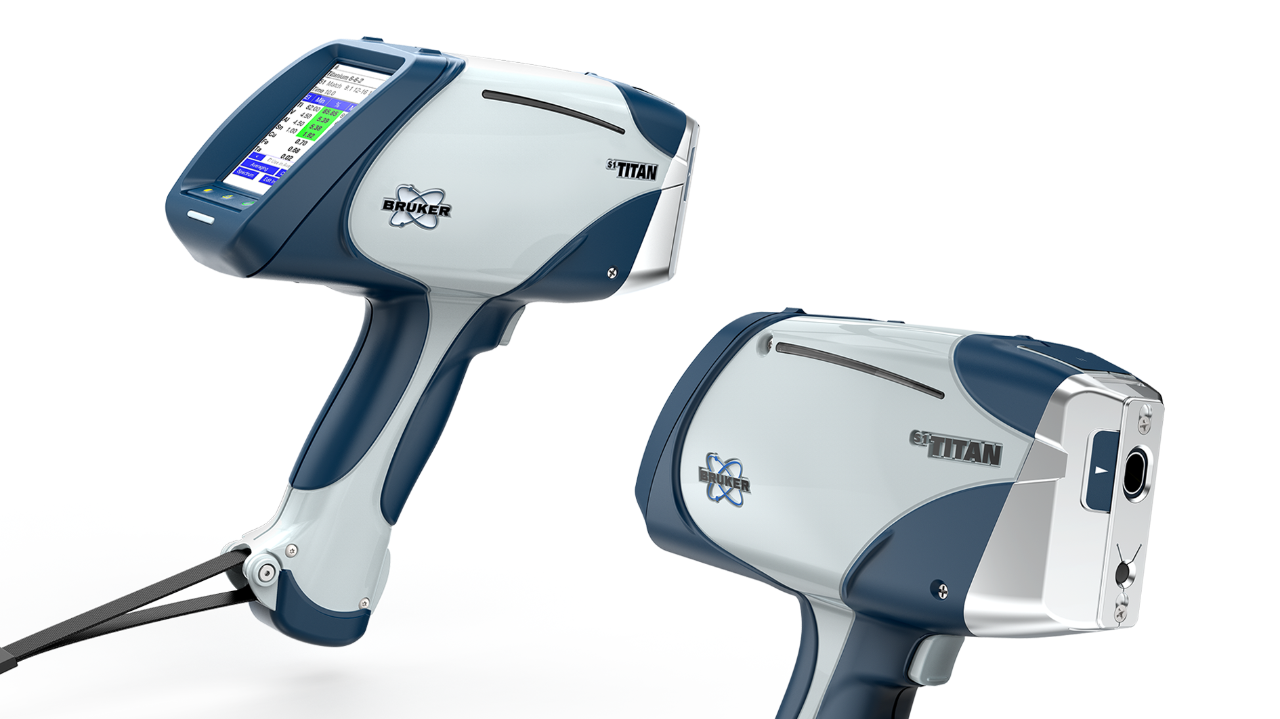
\includegraphics[width=1\textwidth]{img/bruker.png} 
      \caption{Example of handheld XRF scanner. Source: \cite{Bruker}}
      \label{fig:bruker-handheld}
  \end{subfigure}
  \centering     
      \begin{subfigure}{0.45\linewidth}
       \begin{overpic}[width=1\linewidth]{img/ma-xrf.png}
        \put(60,60){\textcolor{black}{X-ray source}}
        \put(25,45){\textcolor{black}{Detector}}
      \end{overpic}
      \caption{MA-XRF spatial imaging concept. Source: \cite{Lach2022}}
      \label{fig:ma-xrf-concept}
  \end{subfigure}
      \caption{Scanning single point}
    \label{fig:ma-xrf}
\end{figure}

Most popular spatial imaging technique involve scanning the object point by point. 
It goes under a name of MA-XRF (Macro X-Ray Fluorescence) and/or $\mu$-XRF (Micro X-Ray Fluorescence), depending on whether the resolution is closer to the range of micrometers ($\sim$100$\mu$m) or millimeters ($\sim$500$\mu$m).

This method comes with crucial disadvantage, as it is sensitive to changes in distance from polycapillary lens that focuses X-rays.
When the distance changes, the resolution also changes, leading to serious distortions in measurements.
Scanning point by point also comes with long measurement time. 
For example, scanning a painting with an area of $65 \times 45$ $\text{cm}^{2}$, a resolution of $1300 \times 900$ pixels (each pixel 500$\mu$m in size), and a dwell time of $10$ ms per pixel could take about $3.5$ hours \cite{Alfeld2013}. 

On the brighter side, it doesn't require high sensitivity for position, has very high energetic resolution, allowing trouble-free identification of elements, and is commonly available (as for scientific equipment).

Due to the demand for eliminating weaknesses in MA-XRF, an alternative method has been developed - FF-XRF (Full-Field X-Ray Fluorescence). 
It is characterized by replacing polycapillary optics with a wide, homogenous beam of radiation paired with pinhole camera. 
This combination guarantees the highest possible (in theory infinite) depth of field, enabling the scanning of uneven surfaces and 3D objects. 
When combined with good position-sensitive detector, it allows for scanning multiple points of surface simultaneously.
However, in contrary to the MA-XRF, choosing the right detector is very tricky.
Detectors with good spatial resolution are in general worse when in comes to the energetic resolution.
For this specific use case, choosing the best detector was challenging, but in the end, it was decided to use slightly modified GEM (Gas Electron Multiplier) detector - \prettyref{fig:ff-xrf}.

\begin{figure}[h] 
  \centering     
      \begin{subfigure}{0.5\linewidth}
      \includegraphics[width=1\textwidth]{img/detart.png} 
      \caption{Prototype FF-XRF scanner. Robotic arm allows for scanning predefined parts of an object.  Source: \cite{Lach2022}}
      \label{fig:ff-xrf-prototype}
  \end{subfigure}
  \centering     
      \begin{subfigure}{0.5\linewidth}
       \begin{overpic}[width=1\linewidth]{img/ff-xrf.png}
        \put(25,85){\textcolor{black}{X-ray source I}}
        \put(30,5){\textcolor{black}{X-ray source II}}
        \put(30,55){\textcolor{black}{Pinhole camera}}
        \put(5,20){\textcolor{black}{Detector}}
      \end{overpic}
      \caption{FF-XRF spatial imaging concept. Source: \cite{Lach2022}}
      \label{fig:ff-xrf-concept}
  \end{subfigure}
  \caption{Scanning multiple points}
  \label{fig:ff-xrf}
\end{figure}